% !TeX encoding = UTF-8
% !TeX program = xelatex
% !TeX spellcheck = en_US

\documentclass[degree=master]{thuthesis}
  % 学位 degree:
  %   doctor | master | bachelor | postdoc
  % 学位类型 degree-type:
  %   academic(默认)| professional


% 论文基本配置,加载宏包等全局配置
% !TeX root = ./thuthesis-example.tex

% 论文基本信息配置

\thusetup{
  %******************************
  % 注意:
  %   1. 配置里面不要出现空行
  %   2. 不需要的配置信息可以删除
  %   3. 建议先阅读文档中所有关于选项的说明
  %******************************
  %
  % 输出格式
  %   选择打印版(print)或用于提交的电子版(electronic),前者会插入空白页以便直接双面打印
  %
  output = electronic,
  language = english,
  font = times,
  %
  % 标题
  %   可使用“\\”命令手动控制换行
  %
  title  = {基于信息瓶颈的表征学习方法},
  title* = {Information Bottleneck for Representation Learning: New Vision},
  %
  % 学位
  %   1. 学术型
  %      - 中文
  %        需注明所属的学科门类,例如:
  %        哲学、经济学、法学、教育学、文学、历史学、理学、工学、农学、医学、
  %        军事学、管理学、艺术学
  %      - 英文
  %        博士:Doctor of Philosophy
  %        硕士:
  %          哲学、文学、历史学、法学、教育学、艺术学门类,公共管理学科
  %          填写“Master of Arts“,其它填写“Master of Science”
  %   2. 专业型
  %      直接填写专业学位的名称,例如:
  %      教育博士、工程硕士等
  %      Doctor of Education, Master of Engineering
  %   3. 本科生不需要填写
  %
  degree-name  = {工学硕士},
  degree-name* = {Master of Science},
  %
  % 培养单位
  %   填写所属院系的全名
  %
  department = {清华伯克利深圳学院},
  %
  % 学科
  %   1. 学术型学位
  %      获得一级学科授权的学科填写一级学科名称,其他填写二级学科名称
  %   2. 工程硕士
  %      工程领域名称
  %   3. 其他专业型学位
  %      不填写此项
  %   4. 本科生填写专业名称,第二学位论文需标注“(第二学位)”
  %
  discipline  = {数据科学与信息技术},
  discipline* = {Data Science and Information Technology},
  %
  % 姓名
  %
  author  = {王子丰},
  author* = {Wang Zifeng},
  %
  % 指导教师
  %   中文姓名和职称之间以英文逗号“,”分开,下同
  %
  supervisor  = {黄绍伦, 副教授},
  supervisor* = {Professor Huang Shao-Lun},
  %
  % 副指导教师
  %
  associate-supervisor  = {Khalid M. Mosalam, 教授},
  associate-supervisor* = {Professor Khalid M. Mosalam},
  %
  % 联合指导教师
  %
  % joint-supervisor  = {某某某, 教授},
  % joint-supervisor* = {Professor Mou Moumou},
  %
  % 日期
  %   使用 ISO 格式;默认为当前时间
  %
  % date = {2019-07-07},
  %
  % 是否在中文封面后的空白页生成书脊(默认 false)
  %
  include-spine = false,
  %
  % 密级和年限
  %   秘密, 机密, 绝密
  %
  % secret-level = {秘密},
  % secret-year  = {10},
  %
  % 博士后专有部分
  %
  % clc                = {分类号},
  % udc                = {UDC},
  % id                 = {编号},
  % discipline-level-1 = {计算机科学与技术},  % 流动站(一级学科)名称
  % discipline-level-2 = {系统结构},          % 专业(二级学科)名称
  % start-date         = {2011-07-01},        % 研究工作起始时间
}

% 载入所需的宏包

% 可以使用 nomencl 生成符号和缩略语说明
% \usepackage{nomencl}
% \makenomenclature

% 表格加脚注
\usepackage{threeparttable}

% 表格中支持跨行
\usepackage{multirow}

% 固定宽度的表格。放在 hyperref 之前的话,tabularx 里的 footnote 显示不出来。
% \usepackage{tabularx}

% 跨页表格
% \usepackage{longtable}

% 量和单位
\usepackage{siunitx}

% 定理类环境宏包
\usepackage{amsthm}
% 也可以使用 ntheorem
% \usepackage[amsmath,thmmarks,hyperref]{ntheorem}

% 参考文献使用 BibTeX + natbib 宏包
% 顺序编码制
\usepackage[sort]{natbib}
\bibliographystyle{thuthesis-numeric}


% 著者-出版年制
% \usepackage{natbib}
% \bibliographystyle{thuthesis-author-year}

% 本科生参考文献的著录格式
% \usepackage[sort]{natbib}
% \bibliographystyle{thuthesis-bachelor}

% 参考文献使用 BibLaTeX 宏包
% \usepackage[backend=biber,style=thuthesis-numeric]{biblatex}
% \usepackage[backend=biber,style=thuthesis-author-year]{biblatex}
% \usepackage[backend=biber,style=apa]{biblatex}
% \usepackage[backend=biber,style=mla-new]{biblatex}
% 声明 BibLaTeX 的数据库
% \addbibresource{ref/refs.bib}

% 定义所有的图片文件在 figures 子目录下
\graphicspath{{figures/}}

% 数学命令
\setmathfont{XITS Math}[
  Scale = MatchUppercase ]
\setmathfont{Latin Modern Math}[
  range = {cal,bfcal},
  Scale = MatchUppercase ]

\newcommand\dif{\mathop{}\!\mathrm{d}}  % 微分符号

% hyperref 宏包在最后调用
\usepackage{hyperref}



\begin{document}

% 封面
\maketitle

% 学位论文指导小组、公开评阅人和答辩委员会名单
\input{data/committee}

% 使用授权的说明
\copyrightpage
% 将签字扫描后授权文件 scan-copyright.pdf 替换原始页面
% \copyrightpage[file=scan-copyright.pdf]

\frontmatter
\input{data/abstract}

% 目录
\tableofcontents

% 插图和附表清单
\listoffiguresandtables  % 插图和附表清单
% \listoffigures           % 插图清单
% \listoftables            % 附表清单

% 符号对照表
% !TeX root = ../thuthesis-example.tex

\begin{denotation}[3cm]
  \item[${\rm \mathbf{A}}$] Matrix
  \item[$\mathbf{a}$] Vector
  \item[$a$] Scalar
  \item[${\rm \mathbf{W}}$] Weight matrix
  \item[$\omega$] A set of random variables $\{{\rm \mathbf{W}}_1, \dots, {\rm \mathbf{W}}_L\}$
  \item[$f^\omega$] Function parametrized by the variables $\omega$
  \item[$S$] Dataset
  \item[${\rm \mathbf{X}}$] Dataset inputs (matrix with $N$ rows, one for each sample)
  \item[${\rm \mathbf{Y}}$] Dataset outputs (matrix with $N$ rows, one for each sample)
  \item[$\mathbf{x}_i$] Input sample for model
  \item[$\mathbf{y}_i$] Output label for model
  \item[$\mathbf{z}_i$] Data point combining both input and output $(\mathbf{x}_i,\mathbf{y}_i)$
  \item[$\hat{\mathbf{y}}_i$] Model prediction on input sample $\mathbf{x}_i$
  \item[$\ell$] Loss function
  \item[$\mathcal{N}$] The Gaussian distribution
  \item[$\mathbb{R}$] The real numbers
  \item[IB] Information bottleneck
  \item[BNN] Bayesian neural network
  \item[VI] Variational inference
  \item[ELBO] Evidence lower bound
  \item[KL] Kullback–Leibler
  \item[DNN] Deep neural network
  \item[MC] Monte Carlo
  \item[MCMC] Markov chain Monte Carlo
  \item[MDL] Minimum description length
  \item[PAC] Probably approximately correct 
  \item[e.g.] Exempli gratia (“for the sake of an example”)
  \item[i.e.] Id est (“it is”)
  \item[i.i.d.] Independent and identically distributed
  \item[s.t.] Subject to
  \item[w.r.t.] With respect to
\end{denotation}



% \printnomenclature[3cm]
% asgsaf

% 也可以使用 nomencl 宏包,需要在导言区
% \usepackage{nomencl}
% \makenomenclature

% 在这里输出符号说明
% \printnomenclature[3cm]

% 在正文中的任意为都可以标题
% \nomenclature{PI}{聚酰亚胺}
% \nomenclature{MPI}{聚酰亚胺模型化合物,N-苯基邻苯酰亚胺}
% \nomenclature{PBI}{聚苯并咪唑}
% \nomenclature{MPBI}{聚苯并咪唑模型化合物,N-苯基苯并咪唑}
% \nomenclature{PY}{聚吡咙}
% \nomenclature{PMDA-BDA}{均苯四酸二酐与联苯四胺合成的聚吡咙薄膜}
% \nomenclature{MPY}{聚吡咙模型化合物}
% \nomenclature{As-PPT}{聚苯基不对称三嗪}
% \nomenclature{MAsPPT}{聚苯基不对称三嗪单模型化合物,3,5,6-三苯基-1,2,4-三嗪}
% \nomenclature{DMAsPPT}{聚苯基不对称三嗪双模型化合物(水解实验模型化合物)}
% \nomenclature{S-PPT}{聚苯基对称三嗪}
% \nomenclature{MSPPT}{聚苯基对称三嗪模型化合物,2,4,6-三苯基-1,3,5-三嗪}
% \nomenclature{PPQ}{聚苯基喹噁啉}
% \nomenclature{MPPQ}{聚苯基喹噁啉模型化合物,3,4-二苯基苯并二嗪}
% \nomenclature{HMPI}{聚酰亚胺模型化合物的质子化产物}
% \nomenclature{HMPY}{聚吡咙模型化合物的质子化产物}
% \nomenclature{HMPBI}{聚苯并咪唑模型化合物的质子化产物}
% \nomenclature{HMAsPPT}{聚苯基不对称三嗪模型化合物的质子化产物}
% \nomenclature{HMSPPT}{聚苯基对称三嗪模型化合物的质子化产物}
% \nomenclature{HMPPQ}{聚苯基喹噁啉模型化合物的质子化产物}
% \nomenclature{PDT}{热分解温度}
% \nomenclature{HPLC}{高效液相色谱 (High Performance Liquid Chromatography)}
% \nomenclature{HPCE}{高效毛细管电泳色谱 (High Performance Capillary lectrophoresis)}
% \nomenclature{LC-MS}{液相色谱-质谱联用 (Liquid chromatography-Mass Spectrum)}
% \nomenclature{TIC}{总离子浓度 (Total Ion Content)}
% \nomenclature{\textit{ab initio}}{基于第一原理的量子化学计算方法,常称从头算法}
% \nomenclature{DFT}{密度泛函理论 (Density Functional Theory)}
% \nomenclature{$E_a$}{化学反应的活化能 (Activation Energy)}
% \nomenclature{ZPE}{零点振动能 (Zero Vibration Energy)}
% \nomenclature{PES}{势能面 (Potential Energy Surface)}
% \nomenclature{TS}{过渡态 (Transition State)}
% \nomenclature{TST}{过渡态理论 (Transition State Theory)}
% \nomenclature{$\increment G^\neq$}{活化自由能(Activation Free Energy)}
% \nomenclature{$\kappa$}{传输系数 (Transmission Coefficient)}
% \nomenclature{IRC}{内禀反应坐标 (Intrinsic Reaction Coordinates)}
% \nomenclature{$\nu_i$}{虚频 (Imaginary Frequency)}
% \nomenclature{ONIOM}{分层算法 (Our own N-layered Integrated molecular Orbital and molecular Mechanics)}
% \nomenclature{SCF}{自洽场 (Self-Consistent Field)}
% \nomenclature{SCRF}{自洽反应场 (Self-Consistent Reaction Field)}



% 正文部分
\mainmatter
% !TeX root = ../thuthesis-example.tex


%\chapter{论文主要部分的写法}
\chapter{Introduction}

\section{Background}
Representation learning \cite{bengio2013representation}, especially deep representation learning (or deep learning, DL), has become one of the most popular techniques since \citet{krizhevsky2012imagenet} developed a powerful deep neural network (DNN) that can significantly outperform shallow methods on ImageNet \cite{deng2009imagenet}. After that, DNN based methods have thrived in various machine learning domains, including computer vision \cite{simonyan2014very}, natural language processing \cite{kim-2014-convolutional}, recommendation \cite{cheng2016wide}, reinforcement learning \cite{silver2016mastering}, and so on. These works make a substantial progress in building better artifical intelligence (AI) applications by DNN. However, it remains elusive why DNN gains so much improvement with adding more layers of representations. This question encourages us to think of opening the black box of DNN.

In statistical learning theory \cite{vapnik2013nature} and probably approximately correct (PAC) learning theory \cite{valiant1984theory}, a too complex model suffers from \emph{over-fitting} problem thus failing in out-of-sample test. Recent work challenged them when the so-called benign over-fitting is observed in practice. That is, a hierarchical representation learning model with the number of parameters much more than the samples, i.e., \emph{over-parametrized}, still generalizes well on numerous tasks. This phenomenon ignites a surge of research under the theme of rethinking the generalization of representation learning \cite{zhang2016understanding}. One pitfall of the traditional learning theory is the lacking consideration of the input data distribution. 

Information theory \cite{cover1999elements} is a promising candidate for unveiling the black box in representation learning. A landmark in this line of research is using information bottleneck (IB) to model the learning process of DNN \cite{tishby2000information, tishby2015deep}. They utilized mutual information between the layers and the input and output variables to quantify DNN. It sheds light on characterizing generalization of representation learning by taking data distribution into account. After that, experiments showed that stochastic gradient descent (SGD) is capable of improving the generalization by compressing the redundant information contained in representations through the lens of IB \cite{shwartz2017opening}.

In information theory, IB was originally proposed as a means of finding minimal sufficient statistics. The minimality term in IB originates from the principle of minimum description length. In the sense of representation learning, IB describes a trade-off between the representation minimality and sufficiency.  The minimality term naturally works for a regularization term that urges the representation to generalize better. This property encourages a series of works in adopting IB for better representation learning. For example, by parameterizing the IB by variational inference, variational information bottleneck was proposed for yielding better generalization performance and robustness to adversarial attack of DNN in image classification \cite{alemi2016deep}. For this reason, it is quite surprising to see how IB could be used for more applications beyond the simple image classification task. In fact, we shall see that we can utilize IB for debasing recommender system models with a novel VI based approach. 

Moreover, in this paper, we explore a new perspective of information bottleneck. We look into a novel information-theoretic generalization measure that is built upon the mutual information between the learned weight and the selected finite-sample dataset. With this measure, we propose a new information bottleneck, namely PAC-Bayes information bottleneck (PIB), and give an MCMC based solution for approximate inference of the optimal posterior.

\section{Representation learning}
The success of machine learning algorithms heavily relies on the representation of data. Prior to the deep learning era, manual feature engineering is a necessary step for preprocessing the raw data and then completing effective machine learning. Representation learning, on the other hand, advocates to automatic learning of informative data representations when building classifiers or other predictors. These representations are encouraged to be informative to the underlying explanatory factors from inputs. As a result, they are expected to be useful for downstream tasks or further fine-tuned under supervision. Since then, the core concern is that how to design good objective functions for learning data representations.

Deep learning (DL) has drawn a great revolution in AI research in past ten years. While the depth is a key factors of the sucess of DL, it should be noted DL is still a subset of the conception of representation learning, in other words, we would prefer to call deep learning as \emph{deep representation learning} for preciseness. For example, Word2Vec was proposed to reduce the number of parameters required by the the re-use of parameters  \cite{mikolov2013distributed}. Unlike the common deep learning setting, this distributed representation learning paradigm does not have multiple layers.

As the name indicates, one key characteristic of deep learning is its depth. Two high-level ideas are that the deep hierarchical architecture promotes the \emph{re-use} of features and improve the feature \emph{abstraction} at the tail near the final output \cite{bengio2013representation}. When the number of layers grows, the number of possible paths grows exponentially. This feature allows computational efficiency of DNN in the universal approximation of arbitrary functions. That is, using deeper models can reduce the number of units required to represent the desired function and can reduce the amount of generalization error \cite{goodfellow2016deep}. On the other hand, the hierarchy of features enables the composition of fundamental concepts towards abstract objects. Generally, more abstract features are more invariant to the local variation of inputs. The invariance thus allowing the excellent predictive power of learned representations. 

However, beyond this perceptual understanding of DL, there are still questions waiting for answers. For example, why stochastic gradient descent (SGD) can encourage both efficient and effective training of DNNs? To what extent different batch size influences the generalization of the learned DNNs? On account of them, We follow the idea of casting our eyes on another toolkit, e.g., information theory, to help us understand and design representation learning algorithms throughout this paper.


\section{Information bottleneck}
In the learning problem, information theory provides a quantitative notion of ``relevant" information, defined by the mutual information $I(X;Y)$ as
\begin{equation}
    I(X;Y) \triangleq \int \int p(x,y) \log \frac{p(x,y)}{p(x)p(y)} dx dy.
\end{equation}
With the input feature $X$ and the target signal $Y$, our object of interest is to extract the information contained in $X$ that is relevant to the target $Y$ by an intermediate representation $T$, i.e., $I(X;Y)=I(T;Y)$.  It could be seen that a trivial way to obtain all the relevant information is just making $T$ an identical mapping. Under the context of information theory, this is often formulated as a ``rate distortion" problem that characterizes the tradeoff between the size of representation, and the average distortion of the reconstructed signal \cite{cover1999elements}. Apart from the target, we design another target to restrict the irrelevant information by minimizing the mutual information $I(X;T)$. We thus build an optimization problem
\begin{equation} \label{eq:mss}
    \min_T I(T;X), \ \text{s.t.} \ I(T;Y)=I(X;Y).
\end{equation}
By solving this problem, we obtain the \emph{simplest} representation of $X$ while still maintain all relevant information of $Y$. In statistical term, the obtained $T$ is thus called \emph{minimal sufficient statistics} (MSS).

\begin{figure}[t]
  \centering
  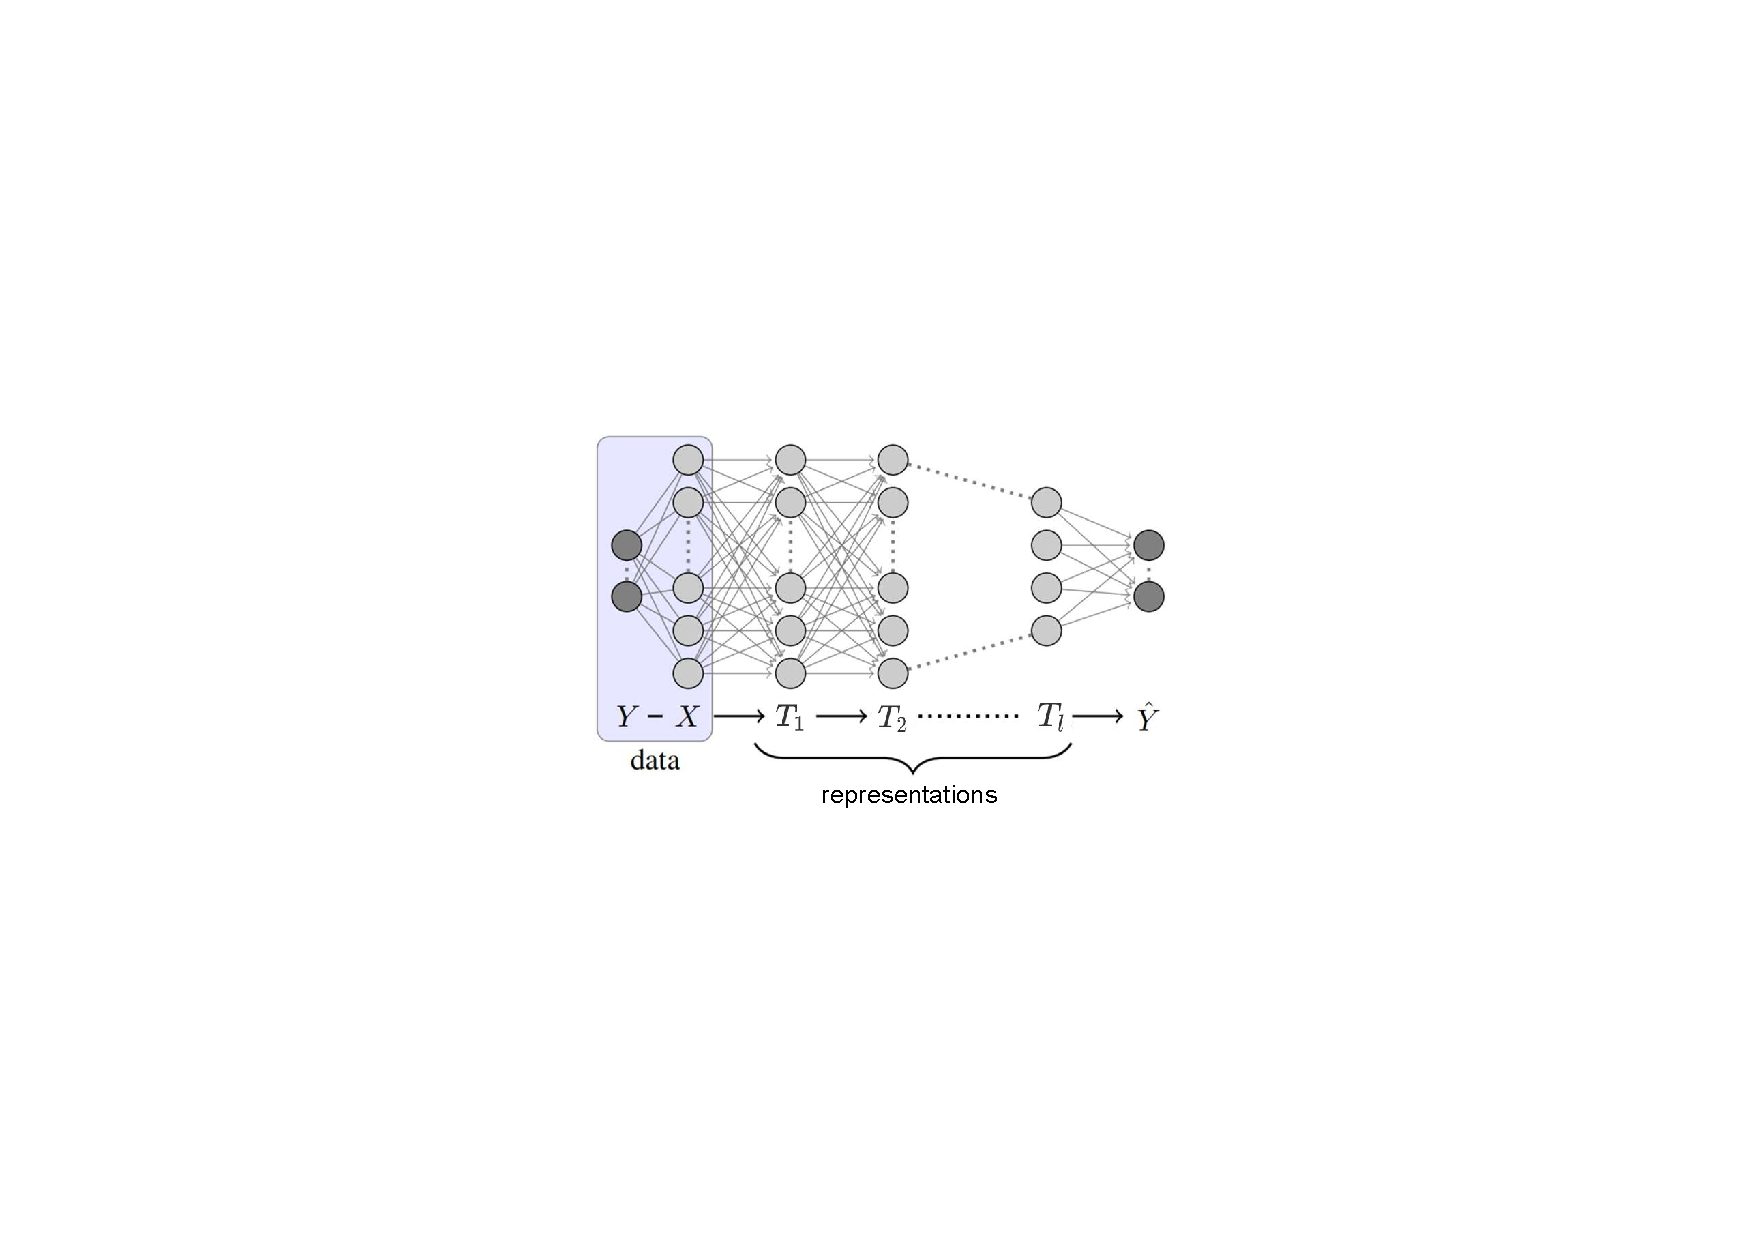
\includegraphics[width=0.6\linewidth]{fig1.pdf}
  \caption{A hierarchy of representations in DNN is formulated as a Markov chain, reproduced from \inlinecite{tishby2015deep}.}
  \label{fig:hierarchy_dnn}
\end{figure}

In this setting, we view the information processing of $X$ as a Markov chain that
\begin{equation}
 Y \to X \to T \to \hat{Y}.
\end{equation}
For a general distribution $p(X,Y)$, however, the MSS might even not exist and the problem in Eq. \eqref{eq:mss} becomes insolvable. On consideration of this challenge, \citet{tishby2000information} proposed a Lagrangian relaxation of the original problem, to build a bottleneck as
\begin{equation}
 \mathcal{L}_{\text{IB}} =  I(X;T) - \beta I(T;Y),
\end{equation}
where $\beta$ is Lagrangian multiplier operates a hyperparameter that controls the tradeoff of regularization and sufficiency.

When there are multiple layers of representations, this Markov chain is also extended such that $X \to T_1 \to T_2 \dots T_l$ as $l$ is the total number of layers, shown by Fig. \ref{fig:hierarchy_dnn}. According to the data processing inequality (DPI), we know that $I(T_1;X) \geq I(T_2;X) \geq \dots I(T_l;X)$.



\emph{in this work we focus on design principled information bottleneck method for representation learning. This method can also be applied for DNN with minimal adaptions in case of computational efficiency.}


\section{Literature review}

\emph{Explaining deep learning through the lens of information}

\section{Thesis structure}


% !TeX root = ../thuthesis-example.tex

% \chapter{图表示例}
\chapter{Variational information bottleneck}
\emph{the mathematical formulation of information bottleneck. also the derivation of variational information bottleneck.}
\section{Summary}
\section{插图}

图片通常在 \env{figure} 环境中使用 \cs{includegraphics} 插入,如图~\ref{fig:example} 的源代码。
建议矢量图片使用 PDF 格式,比如数据可视化的绘图;
照片应使用 JPG 格式;
其他的栅格图应使用无损的 PNG 格式。
注意,LaTeX 不支持 TIFF 格式;EPS 格式已经过时。

\begin{figure}
  \centering
  \includegraphics[width=0.6\linewidth]{example-image-a.pdf}
  \caption{示例图片}
  \label{fig:example}
\end{figure}

若图或表中有附注,采用英文小写字母顺序编号,附注写在图或表的下方。
% LaTeX 传统上一般将附注的内容同图表的标题写在一起,形成很长的一段文字。

如果一个图由两个或两个以上分图组成时,各分图分别以(a)、(b)、(c)...... 作为图序,并须有分图题。
推荐使用 \pkg{subcaption} 宏包来处理, 比如图~\ref{fig:subfig-a} 和图~\ref{fig:subfig-b}。

\begin{figure}
  \centering
  \subcaptionbox{分图 A\label{fig:subfig-a}}
    {\includegraphics[width=0.45\linewidth]{example-image-a.pdf}}
  \subcaptionbox{分图 B\label{fig:subfig-b}}
    {\includegraphics[width=0.45\linewidth]{example-image-b.pdf}}
  \caption{多个分图的示例}
  \label{fig:multi-image}
\end{figure}



\section{表格}

表应具有自明性。为使表格简洁易读,尽可能采用三线表,如表~\ref{tab:three-line}。
三条线可以使用 \pkg{booktabs} 宏包提供的命令生成。

\begin{table}
  \centering
  \caption{三线表示例}
  \begin{tabular}{ll}
    \toprule
    文件名          & 描述                         \\
    \midrule
    thuthesis.dtx   & 模板的源文件,包括文档和注释 \\
    thuthesis.cls   & 模板文件                     \\
    thuthesis-*.bst & BibTeX 参考文献表样式文件    \\
    thuthesis-*.bbx & BibLaTeX 参考文献表样式文件  \\
    thuthesis-*.cbx & BibLaTeX 引用样式文件        \\
    \bottomrule
  \end{tabular}
  \label{tab:three-line}
\end{table}

表格如果有附注,尤其是需要在表格中进行标注时,可以使用 \pkg{threeparttable} 宏包。
研究生要求使用英文小写字母 a、b、c……顺序编号,本科生使用圈码 ①、②、③……编号。

\begin{table}
  \centering
  \begin{threeparttable}[c]
    \caption{带附注的表格示例}
    \label{tab:three-part-table}
    \begin{tabular}{ll}
      \toprule
      文件名                 & 描述                         \\
      \midrule
      thuthesis.dtx\tnote{a} & 模板的源文件,包括文档和注释 \\
      thuthesis.cls\tnote{b} & 模板文件                     \\
      thuthesis-*.bst        & BibTeX 参考文献表样式文件    \\
      thuthesis-*.bbx        & BibLaTeX 参考文献表样式文件  \\
      thuthesis-*.cbx        & BibLaTeX 引用样式文件        \\
      \bottomrule
    \end{tabular}
    \begin{tablenotes}
      \item [a] 可以通过 xelatex 编译生成模板的使用说明文档;
        使用 xetex 编译 \file{thuthesis.ins} 时则会从 \file{.dtx} 中去除掉文档和注释,得到精简的 \file{.cls} 文件。
      \item [b] 更新模板时,一定要记得编译生成 \file{.cls} 文件,否则编译论文时载入的依然是旧版的模板。
    \end{tablenotes}
  \end{threeparttable}
\end{table}

% !TeX root = ../thuthesis-example.tex

\chapter{When Information Bottleneck Meets Counterfactuals}
% \chapter{数学符号和公式}
\section{Summary}
\section{数学符号}

研究生《写作指南》要求量及其单位所使用的符号应符合国家标准《国际单位制及其应用》(GB 3100—1993)、《有关量、单位和符号的一般原则》(GB/T 3101—1993) 的规定。
模板中使用 \pkg{unicode-math} 宏包来配置数学符号,
与 \LaTeX{} 默认的英美国家的符号习惯有所差异:
\begin{enumerate}
  \item 大写希腊字母默认为斜体,如 \cs{Delta}:$\Delta$。
  \item 有限增量符号 $\increment$(U+2206)应使用 \pkg{unicode-math} 宏包提供的
    \cs{increment} 命令。
  \item 向量、矩阵和张量要求粗斜体,应该使用 \pkg{unicode-math} 的 \cs{symbf} 命令,
    如 \verb|\symbf{A}|、\verb|\symbf{\alpha}|。
  \item 数学常数和特殊函数要求用正体,应使用 \cs{symup} 命令,
    如 $\symup{\pi} = 3.14\dots$; $\symup{e} = 2.718\dots$,
  \item 微分号和积分号使用使用正体,比如 $\int f(x) \dif x$。
\end{enumerate}

关于数学符号更多的用法,参考
\href{http://mirrors.ctan.org/macros/latex/contrib/unicode-math/unicode-math.pdf}{\pkg{unicode-math}}
宏包的使用说明,
全部数学符号命的令参考
\href{http://mirrors.ctan.org/macros/latex/contrib/unicode-math/unimath-symbols.pdf}{\pkg{unimath-symbols}}。

关于量和单位推荐使用
\href{http://mirrors.ctan.org/macros/latex/contrib/siunitx/siunitx.pdf}{\pkg{siunitx}}
宏包,
可以方便地处理希腊字母以及数字与单位之间的空白,
比如:
\SI{6.4e6}{m},
\SI{9}{\micro\meter},
\si{kg.m.s^{-1}},
\SIrange{10}{20}{\degreeCelsius}。



\section{数学公式}

数学公式可以使用 \env{equation} 和 \env{equation*} 环境。
注意数学公式的引用应前后带括号,建议使用 \cs{eqref} 命令,比如式 \eqref{eq:example}。
\begin{equation}
  \frac{1}{2 \symup{\pi} \symup{i}} \int_\gamma f = \sum_{k=1}^m n(\gamma; a_k) \mathscr{R}(f; a_k)
  \label{eq:example}
\end{equation}
注意公式编号的引用应含有圆括号,可以使用 \cs{eqref} 命令。

多行公式尽可能在“=”处对齐,推荐使用 \env{align} 环境。
\begin{align}
  a & = b + c + d + e \\
    & = f + g
\end{align}



\section{数学定理}

定理环境的格式可以使用 \pkg{amsthm} 或者 \pkg{ntheorem} 宏包配置。
用户在导言区载入这两者之一后,模板会自动配置 \env{thoerem}、\env{proof} 等环境。

\begin{theorem}[Lindeberg--Lévy 中心极限定理]
  设随机变量 $X_1, X_2, \dots, X_n$ 独立同分布, 且具有期望 $\mu$ 和有限的方差 $\sigma^2 \ne 0$,
  记 $\bar{X}_n = \frac{1}{n} \sum_{i+1}^n X_i$,则
  \begin{equation}
    \lim_{n \to \infty} P \left(\frac{\sqrt{n} \left( \bar{X}_n - \mu \right)}{\sigma} \le z \right) = \Phi(z),
  \end{equation}
  其中 $\Phi(z)$ 是标准正态分布的分布函数。
\end{theorem}
\begin{proof}
  Trivial.
\end{proof}

同时模板还提供了 \env{assumption}、\env{definition}、\env{proposition}、
\env{lemma}、\env{theorem}、\env{axiom}、\env{corollary}、\env{exercise}、
\env{example}、\env{remar}、\env{problem}、\env{conjecture} 这些相关的环境。

% !TeX root = ../thuthesis-example.tex

\chapter{PAC-Bayes Information Bottleneck}
% \chapter{引用文献的标注}

模板支持 BibTeX 和 BibLaTeX 两种方式处理参考文献。
下文主要介绍 BibTeX 配合 \pkg{natbib} 宏包的主要使用方法。

\section{顺序编码制}

在顺序编码制下,默认的 \cs{cite} 命令同 \cs{citep} 一样,序号置于方括号中,
引文页码会放在括号外。
统一处引用的连续序号会自动用短横线连接。

\thusetup{
  cite-style = super,
}
\begin{tabular}{l@{\quad$\Rightarrow$\quad}l}
  \verb|\cite{zhangkun1994}|               & \cite{zhangkun1994}               \\
  \verb|\citet{zhangkun1994}|              & \citet{zhangkun1994}              \\
  \verb|\citep{zhangkun1994}|              & \citep{zhangkun1994}              \\
  \verb|\cite[42]{zhangkun1994}|           & \cite[42]{zhangkun1994}           \\
  \verb|\cite{zhangkun1994,zhukezhen1973}| & \cite{zhangkun1994,zhukezhen1973} \\
\end{tabular}


也可以取消上标格式,将数字序号作为文字的一部分。
建议全文统一使用相同的格式。

\thusetup{
  cite-style = inline,
}
\begin{tabular}{l@{\quad$\Rightarrow$\quad}l}
  \verb|\cite{zhangkun1994}|               & \cite{zhangkun1994}               \\
  \verb|\citet{zhangkun1994}|              & \citet{zhangkun1994}              \\
  \verb|\citep{zhangkun1994}|              & \citep{zhangkun1994}              \\
  \verb|\cite[42]{zhangkun1994}|           & \cite[42]{zhangkun1994}           \\
  \verb|\cite{zhangkun1994,zhukezhen1973}| & \cite{zhangkun1994,zhukezhen1973} \\
\end{tabular}



\section{著者-出版年制}

著者-出版年制下的 \cs{cite} 跟 \cs{citet} 一样。

\thusetup{
  cite-style = author-year,
}
\begin{tabular}{l@{\quad$\Rightarrow$\quad}l}
  \verb|\cite{zhangkun1994}|                & \cite{zhangkun1994}                \\
  \verb|\citet{zhangkun1994}|               & \citet{zhangkun1994}               \\
  \verb|\citep{zhangkun1994}|               & \citep{zhangkun1994}               \\
  \verb|\cite[42]{zhangkun1994}|            & \cite[42]{zhangkun1994}            \\
  \verb|\citep{zhangkun1994,zhukezhen1973}| & \citep{zhangkun1994,zhukezhen1973} \\
\end{tabular}

\vskip 2ex
\thusetup{
  cite-style = super,
}
注意,引文参考文献的每条都要在正文中标注
\cite{zhangkun1994,zhukezhen1973,dupont1974bone,zhengkaiqing1987,%
  jiangxizhou1980,jianduju1994,merkt1995rotational,mellinger1996laser,%
  bixon1996dynamics,mahui1995,carlson1981two,taylor1983scanning,%
  taylor1981study,shimizu1983laser,atkinson1982experimental,%
  kusch1975perturbations,guangxi1993,huosini1989guwu,wangfuzhi1865songlun,%
  zhaoyaodong1998xinshidai,biaozhunhua2002tushu,chubanzhuanye2004,%
  who1970factors,peebles2001probability,baishunong1998zhiwu,%
  weinstein1974pathogenic,hanjiren1985lun,dizhi1936dizhi,%
  tushuguan1957tushuguanxue,aaas1883science,fugang2000fengsha,%
  xiaoyu2001chubanye,oclc2000about,scitor2000project%
}。

% !TeX root = ../thuthesis-example.tex

\chapter{Conclusion and Future Work}

\section{Summary}
\lipsum[2]


% 其他部分
\backmatter

% 参考文献
\bibliography{ref/refs}  % 参考文献使用 BibTeX 编译
% \printbibliography       % 参考文献使用 BibLaTeX 编译

% 附录
\appendix
% \input{data/appendix}
% \input{data/appendix-survey}       % 本科生:外文资料的调研阅读报告
% \input{data/appendix-translation}  % 本科生:外文资料的书面翻译

% 致谢
\input{data/acknowledgements}

% 声明
\statement
% 生成的声明页是否要插入页眉和页脚(默认 empty)
% 仅在需要进行电子签名时,才需要打开这一选项
% 插入的扫描声明页总是会生成页眉(研究生)和页脚,不受这一选项影响
% \statement[page-style=plain]
% 将签字扫描后的声明文件 scan-statement.pdf 替换原始页面
% \statement[file=scan-statement.pdf]

% 个人简历、在学期间完成的相关学术成果
% !TeX root = ../thuthesis-example.tex

\begin{resume}

  \section*{个人简历}

197×年××月××日出生于四川××县。

1992年9月考入××大学化学系××化学专业,1996年7月本科毕业并获得理学学士学位。

1996年9月免试进入清华大学化学系攻读××化学博士至今。

  \section*{在学期间完成的相关学术成果}

  \subsection*{学术论文}

  \begin{achievements}
    \item \textbf{Yang Y}, Ren T L, Zhang L T, et al. Miniature microphone with silicon- based ferroelectric thin films. Integrated Ferroelectrics, 2003, 52:229-235. (SCI收录, 检索号:758FZ.)
    \item \textbf{杨轶}, 张宁欣, 任天令, 等. 硅基铁电微声学器件中薄膜残余应力的研究. 中国机械工程, 2005, 16(14):1289-1291. (EI收录, 检索号:0534931 2907.)
    \item \textbf{杨轶}, 张宁欣, 任天令, 等. 集成铁电器件中的关键工艺研究. 仪器仪表学报, 2003, 24(S4):192-193. (EI源刊.)
    \item \textbf{Yang Y}, Ren T L, Zhu Y P, et al. PMUTs for handwriting recognition. In press. (已被Integrated Ferroelectrics录用. SCI源刊.)
    \item Wu X M, \textbf{Yang Y}, Cai J, et al. Measurements of ferroelectric MEMS microphones. Integrated Ferroelectrics, 2005, 69:417-429. (SCI收录, 检索号:896KM.)
    \item 贾泽, \textbf{杨轶}, 陈兢, 等. 用于压电和电容微麦克风的体硅腐蚀相关研究. 压电与声光, 2006, 28(1):117-119. (EI收录, 检索号:06129773469.)
    \item 伍晓明, \textbf{杨轶}, 张宁欣, 等. 基于MEMS技术的集成铁电硅微麦克风. 中国集成电路, 2003, 53:59-61.
  \end{achievements}


%   \subsection*{专利}

%   \begin{achievements}
%     \item 任天令, 杨轶, 朱一平, 等. 硅基铁电微声学传感器畴极化区域控制和电极连接的方法: 中国, CN1602118A[P]. 2005-03-30.
%     \item Ren T L, Yang Y, Zhu Y P, et al. Piezoelectric micro acoustic sensor based on ferroelectric materials: USA, No.11/215, 102[P]. (美国发明专利申请号.)
%   \end{achievements}

\end{resume}


% 指导教师/指导小组学术评语
% !TeX root = ../thuthesis-example.tex

\chapter{指导小组学术评语}

论文提出了……


% 答辩委员会决议书
% !TeX root = ../thuthesis-example.tex

\chapter{答辩委员会决议书}

论文提出了……

论文取得的主要创新性成果包括:

1. ……

2. ……

3. ……

论文工作表明作者在×××××具有×××××知识,具有××××能力,论文××××,答辩××××。

答辩委员会表决,(×票/一致)同意通过论文答辩,并建议授予×××(姓名)×××(门类)学博士/硕士学位。


% 本科生的综合论文训练记录表(扫描版)
% \record{file=scan-record.pdf}

\end{document}
